% =====================================================================
% TPI — Puestos de hidratación en la Maratón de Buenos Aires (formato paper)
% Universidad Tecnológica Nacional — FRRO — Simulación 2026
%
% OVERLEAF: subir este archivo como main.tex y la carpeta figuras_tpi/
% con sus PNG (o subir Informe_TPI_para_Overleaf.zip). Compilar con pdfLaTeX.
%
% ANTES DE ENTREGAR, completar lo marcado en rojo (\completar{...}):
%   - correos de los autores (Lupo Piatti y Lentino),
%   - link del modelo en AnyLogic Cloud,
%   - link del video en YouTube.
% =====================================================================
\documentclass[11pt,a4paper]{article}

\usepackage[utf8]{inputenc}
\usepackage[T1]{fontenc}
\usepackage{lmodern}
\usepackage{textcomp}
\usepackage[spanish,es-tabla]{babel}
\usepackage{amsmath, amssymb}
\usepackage{graphicx}
\usepackage{booktabs}
\usepackage{geometry}
\usepackage{float}
\usepackage{xcolor}
\usepackage{hyperref}
\usepackage{caption}
\usepackage{array}
\usepackage{titlesec}

\geometry{margin=2.3cm}
\hypersetup{colorlinks=true, linkcolor=blue, urlcolor=blue, citecolor=blue}
\renewcommand{\arraystretch}{1.12}
\newcolumntype{P}[1]{>{\raggedright\arraybackslash}p{#1}}
\captionsetup{font=small, labelfont=bf}
\titleformat{\section}{\large\bfseries}{\thesection.}{0.6em}{}
\titleformat{\subsection}{\normalsize\bfseries}{\thesubsection.}{0.6em}{}
\newcommand{\completar}[1]{\textcolor{red}{#1}}

\begin{document}

% ---------------------------------------------------------------------
\begin{center}
{\LARGE\bfseries Planificación de puestos de hidratación en la\\[2pt]
Maratón de Buenos Aires mediante simulación con datos reales\par}
\vspace{0.5cm}
{\large
Ramiro Ceballos\textsuperscript{1} \quad
Valeria Lupo Piatti\textsuperscript{1} \quad
Magali Lentino\textsuperscript{1}\par}
\vspace{0.25cm}
{\small
\textsuperscript{1}Universidad Tecnológica Nacional, Facultad Regional Rosario — Cátedra de Simulación, 2026\\
\href{mailto:rceballos.work@gmail.com}{rceballos.work@gmail.com} (legajo 46860) ·
\completar{correo} (52868) · \completar{correo} (52109)\par}
\vspace{0.2cm}
{\small Noviembre de 2026\par}
\end{center}

\begin{abstract}
\noindent Los puestos de hidratación de una maratón masiva se planifican hoy por experiencia: se arman todos los puestos y se compra stock de sobra, sin medir cuánto se consume ni qué pasaría con otra configuración. Este trabajo presenta un modelo de simulación de eventos discretos y agentes, construido en AnyLogic, del sistema de hidratación de la Maratón de Buenos Aires 2025. Los 12.792 corredores que terminaron la carrera entran al modelo con su segundo real de largada y su tiempo oficial. Cada uno de los 15 puestos es una cola con voluntarios, inventario propio y reposición por camión. El modelo reproduce el flujo real de corredores por puesto (13 de 15 puestos dentro del $\pm$10\,\%) y el tiempo de carrera (simulado/real $=$ 1,001), y cada corrida llega hasta el último corredor. La decisión de hidratarse de cada corredor depende de su sed, del calor y de cuánto corrió desde su última toma, con intervalos entre tomas según su nivel. Se compararon cuatro escenarios con números aleatorios comunes (20 réplicas, intervalos de confianza del 95\,\%). Un plan ajustado al pronóstico del clima, que arma los puestos, el stock y los voluntarios para la temperatura del día y deja los camiones como respaldo, mantiene la deshidratación por debajo del 0,3\,\% entre 10 y 30\,°C con un costo entre 44 y 54\,\% menor que la configuración real (a 15\,°C, 0,20\,\% de deshidratados y 54\,\% de ahorro). La escasez de recursos deja sin atender al 48\,\% de los que quieren parar, y el exceso pierde \$\,90\,M sin mejorar el servicio de forma apreciable. La configuración real, en cambio, llega al 2,1\,\% de deshidratados a 30\,°C. Si el pronóstico falla por 5\,°C, los camiones de respaldo mantienen la deshidratación en 0,35\,\%; con errores mayores hay que rearmar el plan.

\vspace{0.2cm}
\noindent\textbf{Palabras clave:} simulación de eventos discretos, AnyLogic, maratón, puestos de hidratación, teoría de colas, inventario, números aleatorios comunes.
\end{abstract}

\renewcommand{\abstractname}{Abstract}
\begin{abstract}
\noindent A discrete-event and agent-based AnyLogic model of the hydration system of the 2025 Buenos Aires Marathon was built from real race data (12,792 finishers with their actual start time and official result). The model reproduces the real runner flow at each aid station and the race times. Four scenarios were compared using common random numbers and 95\,\% confidence intervals. A forecast-based plan (stations, stock and volunteers sized for the day's temperature, with backup trucks) keeps dehydration below 0.3\,\% from 10 to 30\,°C at 44--54\,\% lower cost than the real setup, while scarcity causes congestion and excess wastes resources.
\end{abstract}

% ---------------------------------------------------------------------
\section{Introducción}

En las maratones de gran convocatoria, la hidratación de los corredores es a la vez un tema de salud y un problema logístico. Si los puestos quedan lejos entre sí, si faltan voluntarios o si el stock no alcanza, aparecen colas, faltantes y corredores deshidratados. Si sobran recursos, el costo se va en insumos que se compran y no se usan.

La Maratón Internacional de Buenos Aires 2025 tuvo 12.795 inscriptos que largaron, 15 puestos entre el km 5 y el km 40 y un tiempo máximo de 6 horas. La cantidad de puestos, los voluntarios y el stock se deciden con recomendaciones generales y con la experiencia de ediciones anteriores, sin evaluar alternativas. Probar otra configuración en la carrera real no es posible: hay una sola carrera por año y un error afecta la salud de miles de personas.

El sistema combina colas con llegadas muy variables (en el km 5 pasan más de 1.200 corredores por minuto), un inventario con reposición y el estado fisiológico de cada corredor, que depende del clima. Esa combinación no tiene solución analítica cerrada, por lo que se recurre a la simulación \cite{lawkelton,winston}. Este trabajo construye el modelo con los datos reales de la carrera 2025, lo valida contra lo que ocurrió y lo usa para buscar la configuración que hidrata a todos al menor costo.

% ---------------------------------------------------------------------
\section{Objetivos}

\textbf{Objetivo general.} Determinar, mediante simulación con datos reales, la cantidad y ubicación de los puestos, los voluntarios y el stock de bebida y comida que alcanzan para que ningún corredor se deshidrate según las condiciones climáticas, al menor costo posible.

\begin{table}[H]
\centering
\small
\begin{tabular}{lP{6cm}P{7cm}}
\toprule
& \textbf{Objetivo específico} & \textbf{Métrica del modelo} \\
\midrule
O1 & Evitar la deshidratación de los corredores & \% con hidratación mínima menor a 0,7 y \% severos (menor a 0,5) \\
O2 & Asegurar la atención y evitar la congestión & \% de corredores que quisieron parar y no fueron atendidos; espera media y percentil 95 \\
O3 & Evitar los faltantes de insumos & Unidades pedidas sin stock \\
O4 & Minimizar el costo y el desperdicio & Costo total, costo por atención, valor del sobrante y pérdida por exceso \\
O5 & Dimensionar la logística & Ocupación de voluntarios, horas-voluntario y viajes de camión \\
O6 & Medir la robustez frente al clima & Variación de las métricas anteriores con la temperatura del día \\
\bottomrule
\end{tabular}
\caption{Objetivos específicos y métricas con las que se evalúan.}
\end{table}

% ---------------------------------------------------------------------
\section{Metodología}

\subsection{Descripción del sistema y modelo conceptual}

El sistema abarca a los corredores, los 15 puestos, sus voluntarios e insumos, y la reposición desde un depósito. La Tabla~\ref{tab:conceptual} resume cómo se representa cada elemento.

\begin{table}[H]
\centering
\small
\begin{tabular}{lP{12.6cm}}
\toprule
\textbf{Elemento} & \textbf{Representación en el modelo} \\
\midrule
Corredor & Agente con categoría (elite, avanzado, intermedio, principiante), ritmo, hidratación y energía. La hidratación baja con cada km según la necesidad del corredor y el calor, y cada bebida la repone. \\
Puesto & Agente con stock por insumo (agua, isotónica, fruta, gel) y punto de reposición. Cada corredor decide si para; si para, toma un voluntario, es atendido y lo libera. \\
Voluntarios & Servidores de la cola de cada puesto (entre 10 y 35 según el flujo). \\
Recorrido & Movimiento de los corredores sobre el trazado real, en un mapa GIS. \\
Reposición & Camión que viaja por calles reales y operario que descarga hasta la mesa. \\
Clima & Temperatura del día, convertida en un nivel de calor entre 0 y 1 que aumenta la pérdida de hidratación. \\
\bottomrule
\end{tabular}
\caption{Del sistema real al modelo.}
\label{tab:conceptual}
\end{table}

Cada puesto es una cola G/G/$c$: las llegadas surgen del movimiento de los corredores, no son un proceso de Poisson estacionario, y el tiempo de atención es acotado (3 a 9\,s). El inventario es de revisión continua con punto de reposición
\begin{equation}
    ROP = d \cdot L + z \sqrt{d \cdot L},
\end{equation}
donde $d$ es la demanda por minuto medida durante la carrera, $L$ la demora del camión y $z = 1{,}65$ (nivel de servicio del 95\,\%) \cite{silver}.

\textbf{Decisión de hidratarse.} En cada puesto el corredor para con probabilidad
\begin{equation}
    p = \left[ \left( \pi + (1-\pi)\,c(T) \right) \min\!\left(2,\ \frac{\Delta}{I\,(1 - 0{,}5\,c(T))}\right) + 1{,}2\,(1-h) \right] \frac{n}{\tau},
\end{equation}
donde $\pi$ es su propensión a hidratarse con clima fresco, $c(T)$ el nivel de calor del día (entre 0 y 1), $\Delta$ los km que corrió desde su última toma, $I$ su intervalo preferido entre tomas, $h$ su nivel de hidratación, $n$ la necesidad de hidratación de su categoría y $\tau$ su tolerancia al calor. El primer término es el hábito: las ganas de tomar vuelven de a poco después de cada toma, se completan al recorrer el intervalo preferido, siguen creciendo hasta el doble si no toma, y con calor el intervalo se acorta hasta la mitad. El segundo término es la sed por deshidratación. El intervalo depende de la categoría. Los corredores de élite toman \emph{ad libitum} y poco: en total, unos 25\,s de tomar por maratón \cite{beis}. La pauta para recreativos es de 150 a 350\,mL cada 15 a 20 minutos \cite{acsm}, que a su ritmo equivale a 2,5 a 5\,km. Con esta regla, en el escenario base cada corredor toma en promedio 9,5 veces en los 15 puestos. En el km 5 para el 74\,\% de los corredores, pero solo alrededor de un cuarto de los de élite, y nadie pasa muchos puestos seguidos sin tomar. La simulación es terminante: empieza vacía con la largada y termina cuando llega el último corredor (unos 400 minutos a 15\,°C), sin período de calentamiento.

\subsection{Datos y distribuciones}

Se usaron los resultados oficiales públicos de la carrera 2025 \cite{raceresult}: para cada corredor, el segundo en que cruzó la largada, los tiempos parciales cada 5\,km y el tiempo neto final. No se obtuvieron datos internos de la organización. Lo que no se pudo medir se tomó de estudios publicados sobre maratones masivas o quedó como parámetro del modelo (Tabla~\ref{tab:datos}).

\begin{table}[H]
\centering
\small
\begin{tabular}{P{5cm}P{3.6cm}P{2.1cm}P{4.2cm}}
\toprule
\textbf{Dato} & \textbf{Valor} & \textbf{Tipo} & \textbf{Fuente} \\
\midrule
Largada, parciales y tiempo final por corredor & 12.795 (12.792 llegaron) & Real & Resultados oficiales \cite{raceresult} \\
Ubicación y oferta de los puestos & 15 puestos, km 5 a 40 & Real & Mapa oficial del circuito \\
Clima del día & 12--15\,°C en la largada, máx. 18\,°C & Real & Pronóstico del SMN \cite{smn} \\
Ingesta de líquido & 466 $\pm$ 279 mL/h & Bibliografía & \cite{jimenez} \\
Volumen por vaso & 116 mL & Bibliografía & \cite{cheuvront} \\
Voluntarios por puesto & 10 a 35 & Bibliografía & \cite{vermont} \\
Toma de los corredores de élite & $\approx$25\,s de tomar por maratón, \emph{ad libitum} & Bibliografía & \cite{beis} \\
Pauta de hidratación recreativa & 150--350\,mL cada 15--20 min & Bibliografía & \cite{acsm} \\
Consumo de gel y fruta, precios & Valores de ejemplo & Supuesto & Parámetros del modelo \\
\bottomrule
\end{tabular}
\caption{Datos reales, bibliográficos y supuestos.}
\label{tab:datos}
\end{table}

Se ajustaron distribuciones teóricas con la prueba de Kolmogorov-Smirnov. El tiempo neto se ajusta a una lognormal, que no se rechaza al 5\,\% (Figura~\ref{fig:tiempo}). El cruce de la largada no se ajusta a ninguna distribución teórica, porque depende de los corrales de salida, así que el modelo usa la traza empírica: cada corredor entra en su segundo real y corre al ritmo de su tiempo oficial. Así se conserva además la correlación entre la largada y el ritmo (Spearman 0,48). La Tabla~\ref{tab:distribuciones} resume las distribuciones del modelo.

\begin{figure}[H]
    \centering
    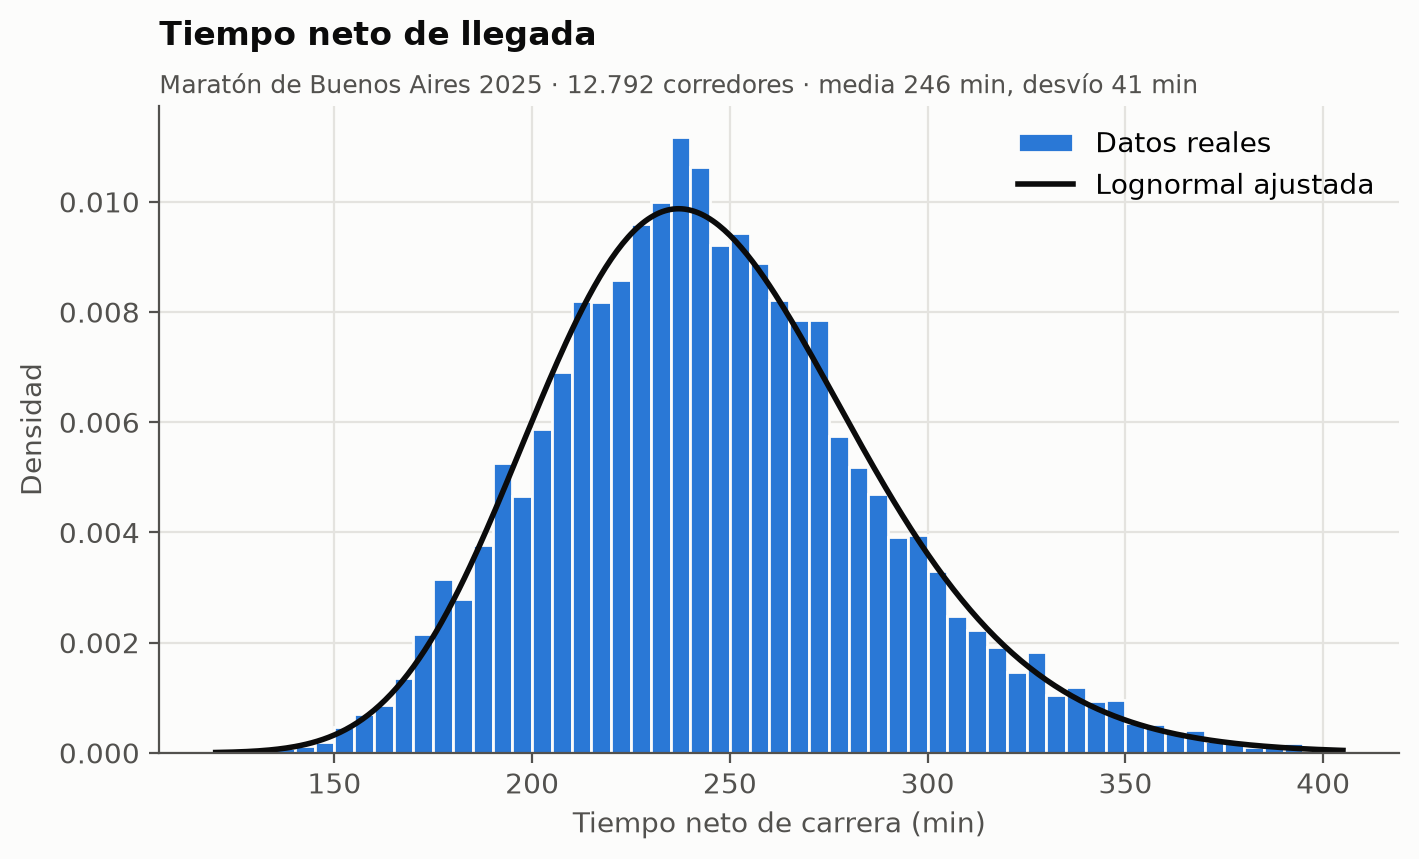
\includegraphics[width=0.72\textwidth]{figuras_tpi/fig1_tiempo_llegada.png}
    \caption{Tiempo neto real de los 12.792 corredores y lognormal ajustada (Kolmogorov-Smirnov: $D = 0{,}011$, $p = 0{,}073$).}
    \label{fig:tiempo}
\end{figure}

\begin{table}[H]
\centering
\small
\begin{tabular}{P{3.4cm}P{2.7cm}P{5cm}P{3.9cm}}
\toprule
\textbf{Elemento} & \textbf{Distribución} & \textbf{Parámetros} & \textbf{Justificación} \\
\midrule
Largada y ritmo & Empírica (traza real) & 12.792 pares (segundo de cruce, tiempo neto) & Reproduce la carrera real \\
Categoría & Derivada del tiempo real & Cortes en 175,0 / 210,9 / 264,7 min (3 / 17 / 50 / 30\,\%) & Define necesidades y comportamiento \\
Tolerancia al calor & Uniforme & Elite $U(1{,}1;\,1{,}4)$ a principiante $U(0{,}7;\,1{,}1)$ & Solo se conoce un rango \\
Propensión a hidratarse & Uniforme & Elite $U(0{,}15;\,0{,}30)$ a principiante $U(0{,}35;\,0{,}55)$ & Rango plausible \\
Tiempo de atención & Uniforme & $U(0{,}05;\,0{,}15)$ min $\times$ factor de categoría & Entregar un vaso: 3 a 9\,s \\
Intervalo entre tomas & Uniforme & Elite $U(8;\,12)$, avanzado $U(5;\,8)$, intermedio $U(3{,}5;\,5{,}5)$, principiante $U(2{,}5;\,4)$ km & Hábito de toma según el nivel \cite{beis,acsm} \\
Decisión de parar & Bernoulli$(p)$ & $p$ según hábito, calor y sed (ecuación de decisión) & Decisión individual \\
Bebida y fruta elegidas & Bernoulli & 0,7 o 0,4 según la categoría & Preferencias supuestas \\
Demanda en la reposición & Poisson & media $=$ varianza $= d \cdot L$ & Stock de seguridad \\
\bottomrule
\end{tabular}
\caption{Distribuciones de probabilidad del modelo.}
\label{tab:distribuciones}
\end{table}

\subsection{Implementación en AnyLogic}

El modelo se construyó en AnyLogic 8.9 (Personal Learning Edition) \cite{grigoryev}. El recorrido de cada corredor por los 15 puestos usa la Process Modeling Library (Source, MoveTo, SelectOutput, Seize, Delay, Release y un ResourcePool de voluntarios por puesto). El mapa, el trazado y el camino de los camiones usan la librería GIS. Una escena 3D de cada puesto, hecha con la Pedestrian Library, muestra a los corredores y a los voluntarios en la calle. Hay 9 tipos de agente: Main, Corredor, Puesto, Camion, OperarioZorra, PuestoDetalle3D, Voluntario, peatonPuesto y Transeunte. La interfaz incluye gráficos en vivo de stock y costos, controles para cambiar voluntarios, stock y precios durante la corrida, y una sección que compara la corrida con la carrera real (Figura~\ref{fig:interfaz}). Las corridas en lote se hacen con experimentos Parameter Variation que exportan cada corrida a CSV. La versión gratuita de AnyLogic corta toda corrida a las 5 horas cuando el modelo usa la Pedestrian Library, y con ese corte quedaban afuera los 1.405 corredores más lentos (11\,\%). Por eso hay dos versiones del modelo con la misma lógica: la completa, con las escenas 3D, para la demostración y AnyLogic Cloud (hasta los 300 min), y una sin las escenas 3D ni la Pedestrian Library, con la que se hicieron todos los experimentos y que simula la carrera hasta el último corredor.

\begin{figure}[H]
    \centering
    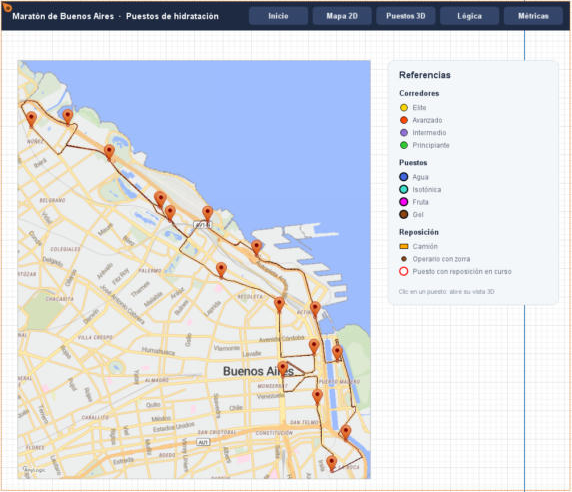
\includegraphics[width=0.55\textwidth]{figuras_tpi/cap_mapa2d.png}
    \caption{Interfaz del modelo: mapa con el recorrido real, los 15 puestos y los corredores por categoría.}
    \label{fig:interfaz}
\end{figure}

\subsection{Verificación y validación}

Para verificar que el modelo hace lo que se pretende se corrieron casos de prueba con un resultado esperado conocido (Tabla~\ref{tab:verificacion}). Todos dieron el resultado esperado.

\begin{table}[H]
\centering
\small
\begin{tabular}{P{3cm}P{4.4cm}P{3.6cm}P{4.2cm}}
\toprule
\textbf{Prueba} & \textbf{Configuración} & \textbf{Esperado} & \textbf{Obtenido} \\
\midrule
Reproducibilidad & Misma semilla dos veces, una de ellas con la vista 3D abierta & Resultados idénticos & Diferencia 0 en todas las métricas \\
Dos versiones del modelo & Con y sin escenas 3D, cortadas a los 300 min (4 escenarios, 2 semillas) & Resultados idénticos & Diferencia 0 en las 35 métricas exportadas \\
Recursos insuficientes & Un cuarto de la dotación y 35\,\% del stock (E2) & Colas, no atendidos y faltantes & 48\,\% de no atendidos y 171 faltantes \\
Más recursos & Doble de voluntarios y stock & El servicio no empeora & Igual o apenas mejor (0,25 puntos menos de no atendidos) \\
Calor & 10 a 30\,°C & Más deshidratación donde los recursos son justos & Crece en E0 y E2; E1 (planificado con el pronóstico) y E3 quedan por debajo del 0,3\,\% \\
\bottomrule
\end{tabular}
\caption{Casos de prueba de verificación.}
\label{tab:verificacion}
\end{table}

Para validar, se comparó la configuración real con lo que pasó en la carrera 2025. El tiempo neto simulado de los 12.792 corredores coincide con el real (246,2 contra 245,8 min; simulado/real $=$ 1,001), con un factor de ajuste de ritmo de 1,039. El flujo de corredores por puesto también coincide (Tabla~\ref{tab:validacion}): 13 de los 15 puestos quedan dentro del $\pm$10\,\% en el pico (los del km 20 y 22,6 quedan en $-$18 y $-$10,4\,\%), y los picos caen en el mismo minuto o con $\pm$4 min de diferencia. El último corredor llega a los 403,6 min de la largada, contra 401,0 min en la realidad.

\begin{table}[H]
\centering
\small
\begin{tabular}{lrrl}
\toprule
\textbf{Puesto (km)} & \textbf{Pico real (corr./min)} & \textbf{Pico simulado} & \textbf{Diferencia} \\
\midrule
1 (km 5) & 1.235 (min 28) & 1.148 (min 28) & $-$7\,\%, mismo minuto \\
3 (km 10) & 627 (min 55) & 627 (min 55) & 0,0\,\%, mismo minuto \\
7 (km 20) & 391 (min 111) & 320 (min 111) & $-$18\,\% (salto aislado en el dato real) \\
11 (km 30) & 248 (min 168) & 224 (min 164) & $-$9,7\,\% \\
15 (km 40) & 165 (min 223) & 168 (min 227) & +2\,\% \\
\bottomrule
\end{tabular}
\caption{Flujo de corredores en el pico: carrera real contra simulación.}
\label{tab:validacion}
\end{table}

\subsection{Diseño de experimentos}

Se definieron cuatro escenarios (Tabla~\ref{tab:escenarios-def}). El escenario base reproduce la configuración real. El optimista (óptimo según el clima) se obtuvo así: la distancia máxima entre dos puestos con bebida es
\begin{equation}
    d_{\max}(T) = \frac{C}{0{,}025 \cdot 1{,}15 \cdot \left(0{,}6 + 0{,}8\,c(T)\right)},
\end{equation}
donde el denominador es la pérdida de hidratación por km del corredor más exigente y $c(T)$ es el nivel de calor a la temperatura pronosticada $T$. El valor teórico $C = 0{,}15$ (poder saltear un puesto) daba 9 puestos, pero el 1,8\,\% de los corredores se deshidrataba, porque a veces se saltean dos o tres seguidos. Por eso $C$ se calibró por simulación con un barrido de $C$ entre 0,090 y 0,150: a 15\,°C el primer plan con menos del 1\,\% de deshidratados es el de 12 puestos (0,24\,\%, con $C = 0{,}114$). El mismo barrido a 10, 20, 25 y 30\,°C (275 corridas en total) confirma que con $C = 0{,}114$ la regla arma 9 puestos a 10\,°C y los 15 desde 20\,°C, siempre con menos del 1\,\% de deshidratados, salvo a 30\,°C, donde el límite pasa a ser la cantidad de voluntarios. El stock de cada puesto e insumo es la demanda observada por corredor (lo retirado más lo que habrían tomado los que no fueron atendidos) más 1,65 desvíos, que cubre el 95\,\% de las carreras, con una tabla por temperatura. Los voluntarios crecen con el calor pronosticado en la misma proporción que los corredores que paran ($\times$1,2 a 20\,°C y $\times$1,5 a 30\,°C). Los camiones quedan de respaldo: salen solo si, con el retiro medido en la carrera, el stock no va a alcanzar hasta el último corredor, y llevan lo que falta.

\begin{table}[H]
\centering
\small
\begin{tabular}{P{3.6cm}P{11.6cm}}
\toprule
\textbf{Escenario} & \textbf{Configuración} \\
\midrule
E0 — Base 2025 & 15 puestos; 10 a 35 voluntarios según el flujo real; stock según la demanda fisiológica; reposición con camión \\
E1 — Optimista (óptimo según el clima) & Puestos según $d_{\max}(T)$ con la temperatura pronosticada (12 puestos a 15\,°C); stock $=$ demanda observada $+\,1{,}65\,\sigma$; voluntarios según el calor; camiones de respaldo \\
E2 — Pesimista (escasez) & 15 puestos, un cuarto de los voluntarios y 35\,\% del stock \\
E3 — Excesivo (exceso de recursos) & 15 puestos, el doble de voluntarios y de stock \\
\bottomrule
\end{tabular}
\caption{Escenarios evaluados. Cada uno tiene su experimento en el modelo: \texttt{Simulation}, \texttt{Optimista}, \texttt{Pesimista} y \texttt{Excesivo}.}
\label{tab:escenarios-def}
\end{table}

Cada escenario se corrió con las semillas 1 a 20, y cada corrida simula la carrera completa. La semilla se fija al inicio de cada corrida, de modo que los cuatro escenarios usan los mismos números aleatorios y se pueden comparar de a pares con la misma semilla. La lógica de la carrera sortea con un generador propio, separado del que usan la animación 3D y la biblioteca de peatones, así que abrir una vista durante la corrida no cambia el resultado. Para cada métrica se calculó el intervalo de confianza del 95\,\%
\begin{equation}
    \bar{x} \pm t_{0{,}975;\,n-1} \, \frac{s}{\sqrt{n}},
\end{equation}
y la diferencia pareada de cada escenario contra E0, que es significativa cuando su intervalo no contiene al cero. La cantidad de réplicas necesaria para un error $e$ se estimó con $n = (t \cdot s / e)^2$. Para el análisis de sensibilidad se varió la temperatura del día entre 10 y 30\,°C; E1 se planificó con esa temperatura (el pronóstico acierta). Aparte, 60 corridas miden qué pasa si el pronóstico falla: E1 armado para 15\,°C en días de 20, 25 y 30\,°C. En total son 4 escenarios $\times$ 20 semillas $\times$ 5 temperaturas $=$ 400 corridas, todas incluidas en la planilla de resultados.

% ---------------------------------------------------------------------
\section{Resultados}

\subsection{Comparación de escenarios}

La Tabla~\ref{tab:escenarios} y la Figura~\ref{fig:escenarios} muestran los escenarios a 15\,°C, la temperatura de la carrera 2025.

\begin{table}[H]
\centering
\small
\begin{tabular}{lrrrr}
\toprule
\textbf{Métrica} & \textbf{E0 Base 2025} & \textbf{E1 Optimista} & \textbf{E2 Pesimista} & \textbf{E3 Excesivo} \\
\midrule
Corredores deshidratados (\%) & 0,08 $\pm$ 0,01 & 0,20 $\pm$ 0,01 & 37,54 $\pm$ 0,17 & 0,09 $\pm$ 0,01 \\
Deshidratación severa (\%) & 0,00 $\pm$ 0,00 & 0,00 $\pm$ 0,00 & 6,74 $\pm$ 0,10 & 0,00 $\pm$ 0,00 \\
No atendidos (\%) & 0,25 $\pm$ 0,01 & 0,31 $\pm$ 0,01 & 47,64 $\pm$ 0,06 & 0,00 $\pm$ 0,00 \\
Espera media en cola (s) & 0,09 $\pm$ 0,00 & 0,11 $\pm$ 0,00 & 1,88 $\pm$ 0,00 & 0,00 $\pm$ 0,00 \\
Espera P95, puesto más exigido (s) & 3,0 $\pm$ 0,0 & 3,0 $\pm$ 0,0 & 5,0 $\pm$ 0,1 & 0,0 $\pm$ 0,0 \\
Unidades faltantes (u) & 0 $\pm$ 0 & 29 $\pm$ 13 & 171 $\pm$ 9 & 0 $\pm$ 0 \\
Ocupación de voluntarios (\%) & 14,6 $\pm$ 0,0 & 16,3 $\pm$ 0,0 & 34,7 $\pm$ 0,0 & 7,4 $\pm$ 0,0 \\
Costo total (M\$) & 119,51 $\pm$ 0,72 & 55,51 $\pm$ 0,03 & 61,35 $\pm$ 0,08 & 143,83 $\pm$ 0,00 \\
Costo por atención (\$) & 988 $\pm$ 6 & 532 $\pm$ 0 & 811 $\pm$ 1 & 1.187 $\pm$ 1 \\
Valor del sobrante (M\$) & 63,47 $\pm$ 0,70 & 3,05 $\pm$ 0,05 & 22,59 $\pm$ 0,04 & 86,75 $\pm$ 0,04 \\
Pérdida por exceso (M\$) & 64,83 $\pm$ 0,70 & 4,11 $\pm$ 0,05 & 22,88 $\pm$ 0,04 & 89,61 $\pm$ 0,04 \\
\bottomrule
\end{tabular}
\caption{Escenarios a 15\,°C: media $\pm$ semiamplitud del intervalo de confianza del 95\,\% (20 réplicas).}
\label{tab:escenarios}
\end{table}

\begin{figure}[H]
    \centering
    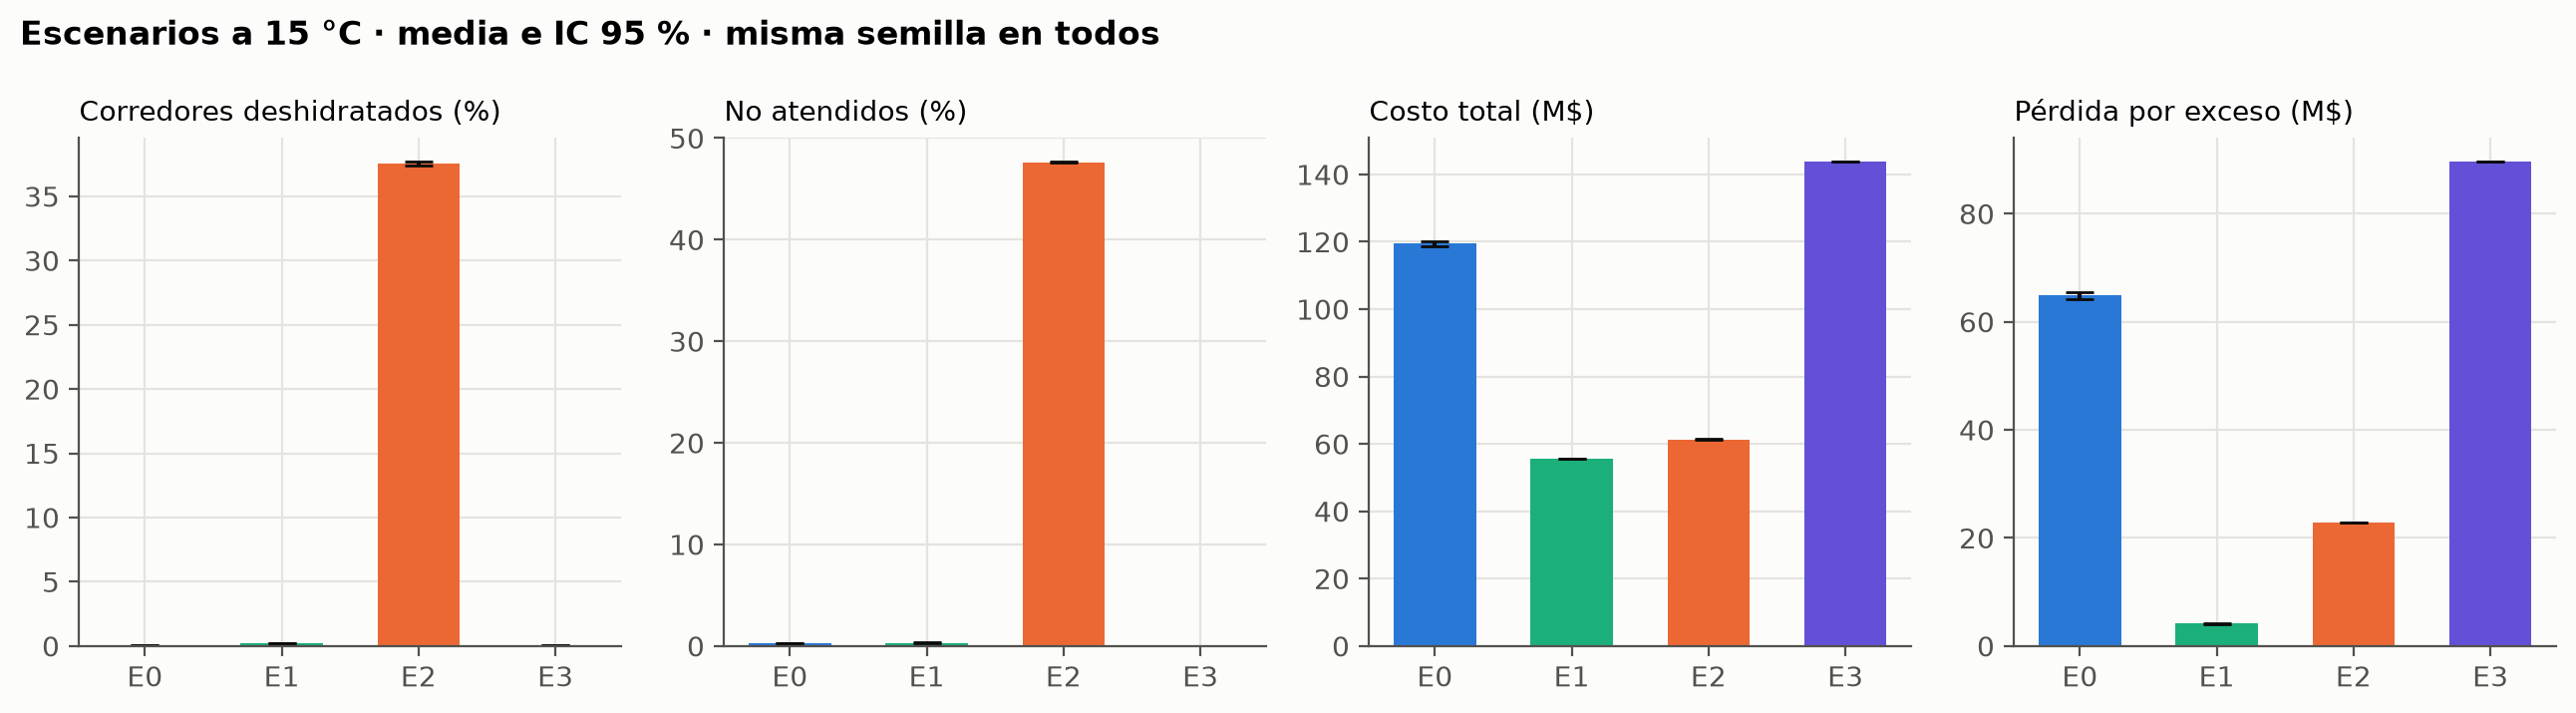
\includegraphics[width=0.95\textwidth]{figuras_tpi/fig5_escenarios_ic.png}
    \caption{Escenarios a 15\,°C con su intervalo de confianza del 95\,\%.}
    \label{fig:escenarios}
\end{figure}

La configuración real (E0) atiende prácticamente a todos (0,25\,\% sin atender, en el pico del km 5) y casi nadie se deshidrata, pero más de la mitad de su costo es sobrante: compra unos \$\,63\,M en insumos que no se consumen. El escenario pesimista (E2) produce la congestión esperada: casi la mitad de los que quieren parar no es atendida, la espera en el puesto más exigido llega a 5,0\,s, faltan 171 unidades y el 38\,\% de los corredores termina deshidratado. El excesivo (E3) apenas atiende mejor que la base, pero cuesta más y pierde \$\,90\,M entre insumos sin usar y horas de voluntarios ociosas.

\subsection{Diferencias pareadas contra la configuración real}

\begin{table}[H]
\centering
\small
\begin{tabular}{lrrr}
\toprule
\textbf{Métrica} & \textbf{E1 $-$ E0} & \textbf{E2 $-$ E0} & \textbf{E3 $-$ E0} \\
\midrule
Corredores deshidratados (\%) & 0,13 $\pm$ 0,01 $^{*}$ & 37,46 $\pm$ 0,17 $^{*}$ & 0,01 $\pm$ 0,01 (ns) \\
No atendidos (\%) & 0,06 $\pm$ 0,01 $^{*}$ & 47,39 $\pm$ 0,05 $^{*}$ & $-$0,25 $\pm$ 0,01 $^{*}$ \\
Espera P95, puesto más exigido (s) & 0,0 $\pm$ 0,0 (ns) & 1,9 $\pm$ 0,1 $^{*}$ & $-$3,0 $\pm$ 0,0 $^{*}$ \\
Unidades faltantes (u) & 29 $\pm$ 13 $^{*}$ & 171 $\pm$ 9 $^{*}$ & 0 $\pm$ 0 (ns) \\
Costo total (M\$) & $-$63,99 $\pm$ 0,71 $^{*}$ & $-$58,16 $\pm$ 0,71 $^{*}$ & 24,32 $\pm$ 0,72 $^{*}$ \\
Pérdida por exceso (M\$) & $-$60,72 $\pm$ 0,69 $^{*}$ & $-$41,95 $\pm$ 0,71 $^{*}$ & 24,78 $\pm$ 0,70 $^{*}$ \\
\bottomrule
\end{tabular}
\caption{Diferencia contra E0 con la misma semilla (intervalo de confianza del 95\,\%). $^{*}$ significativa al 5\,\%; (ns) no significativa.}
\label{tab:diferencias}
\end{table}

Con la misma semilla, el escenario optimista cuesta \$\,64,0\,M menos que la base ($-$54\,\%) y desperdicia \$\,61\,M menos. A cambio, la deshidratación sube 0,13 puntos (de 0,08 a 0,20\,\%): la diferencia es estadísticamente significativa, pero queda muy por debajo del objetivo de menos del 1\,\% y sin casos severos. E3 atiende a todos (0,25 puntos menos de no atendidos, diferencia significativa), pero no cambia la deshidratación (la diferencia no es significativa) y cuesta \$\,24\,M más.

Para fijar la cantidad de réplicas se usó $n = (t \cdot s / e)^2$ con un error aceptado de 0,5 puntos porcentuales en deshidratados y no atendidos y de \$\,1\,M en el costo. Con una primera tanda de 10 réplicas, la deshidratación y los no atendidos pedían como mucho 3 réplicas en las 20 combinaciones de escenario y temperatura, pero el costo de E0 a 15\,°C, que varía más por los viajes de camión, pedía 15. Por eso se llevaron todas las combinaciones a 20 réplicas: con ellas la fórmula pide como máximo 11 (el costo de E0), así que el error queda por debajo del aceptado en todas las métricas. La semiamplitud del costo de E0, de \$\,0,72\,M, es chica frente a las diferencias entre escenarios, de \$\,24\,M o más.

\subsection{Sensibilidad a la temperatura}

La Figura~\ref{fig:sensibilidad} y la Tabla~\ref{tab:sensibilidad} muestran cómo cambian los escenarios con la temperatura del día. E1 se planificó en cada caso con esa temperatura.

\begin{figure}[H]
    \centering
    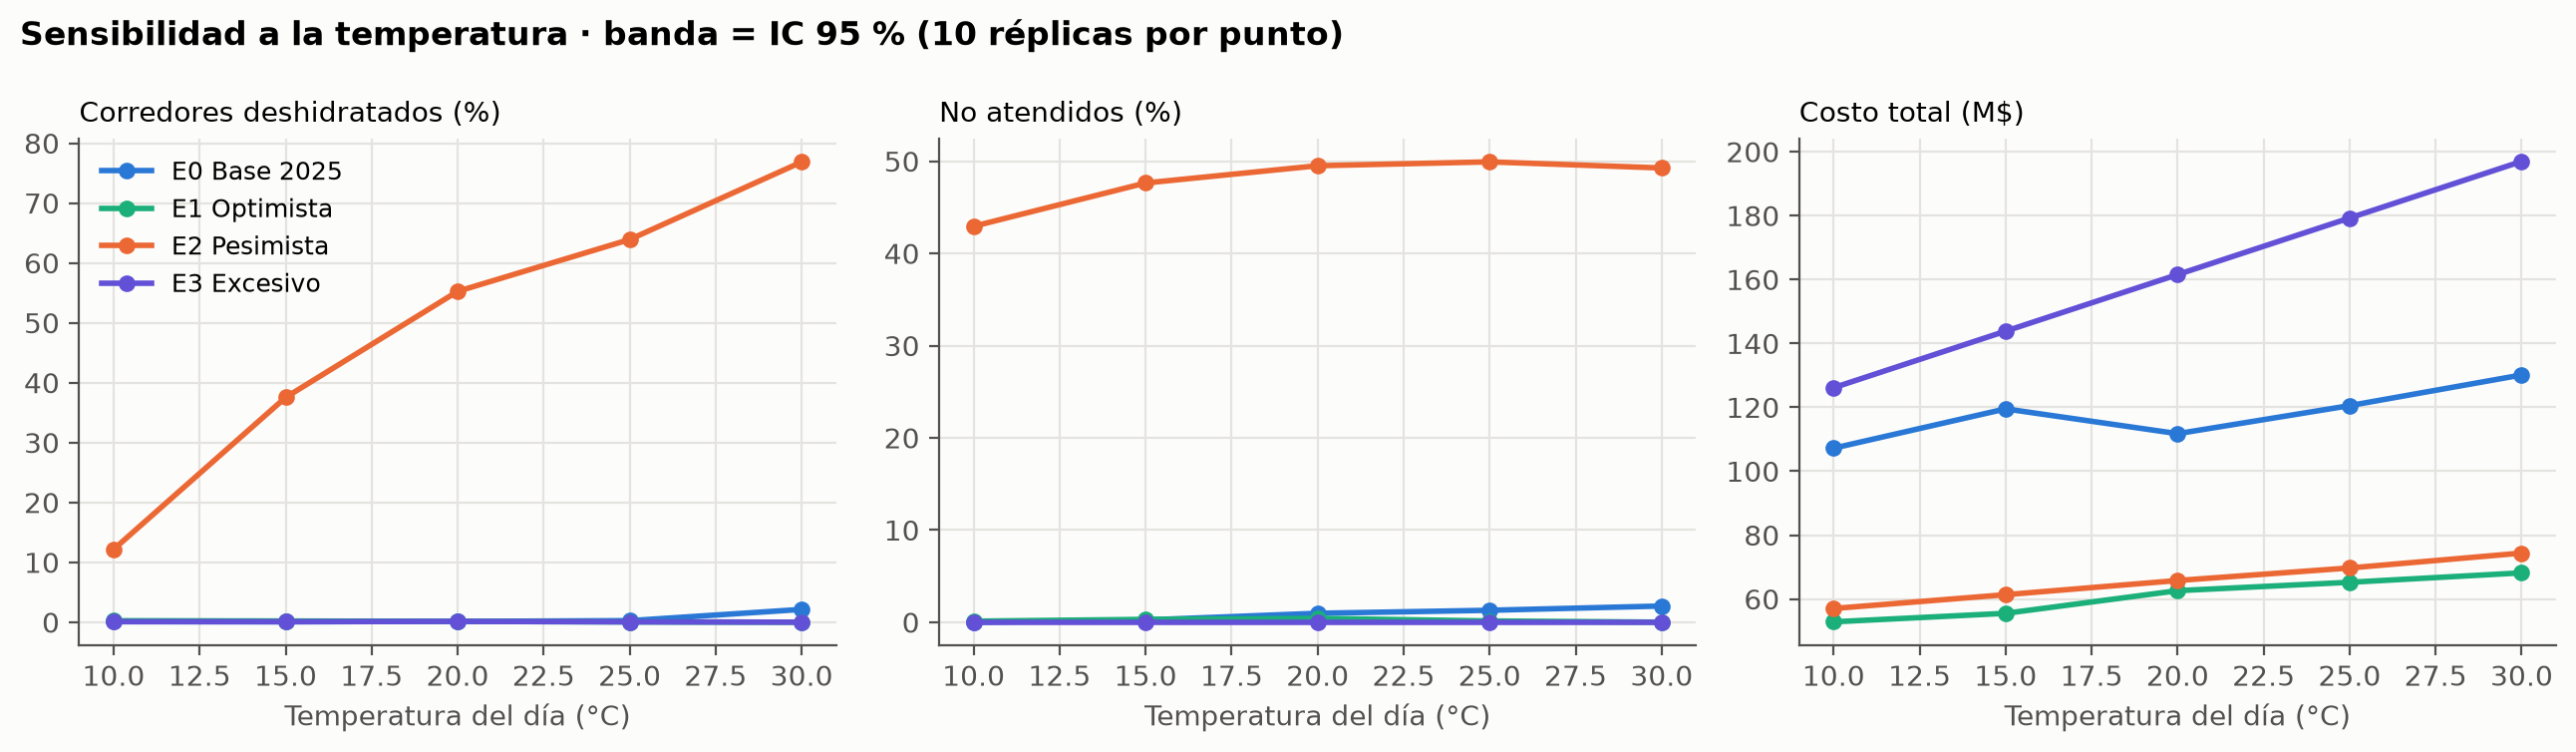
\includegraphics[width=0.95\textwidth]{figuras_tpi/fig6_sensibilidad_temperatura.png}
    \caption{Sensibilidad a la temperatura real del día; la banda es el intervalo de confianza del 95\,\%.}
    \label{fig:sensibilidad}
\end{figure}

\begin{table}[H]
\centering
\small
\begin{tabular}{llrrrrr}
\toprule
\textbf{Métrica} & \textbf{Escenario} & \textbf{10\,°C} & \textbf{15\,°C} & \textbf{20\,°C} & \textbf{25\,°C} & \textbf{30\,°C} \\
\midrule
Deshidratados (\%) & E0 Base & 0,10 $\pm$ 0,01 & 0,08 $\pm$ 0,01 & 0,14 $\pm$ 0,02 & 0,26 $\pm$ 0,02 & 2,14 $\pm$ 0,06 \\
 & E1 Optimista & 0,25 $\pm$ 0,01 & 0,20 $\pm$ 0,01 & 0,14 $\pm$ 0,02 & 0,05 $\pm$ 0,01 & 0,00 $\pm$ 0,01 \\
 & E2 Pesimista & 12,16 $\pm$ 0,12 & 37,54 $\pm$ 0,17 & 55,25 $\pm$ 0,15 & 63,91 $\pm$ 0,12 & 76,86 $\pm$ 0,10 \\
 & E3 Excesivo & 0,09 $\pm$ 0,01 & 0,09 $\pm$ 0,01 & 0,13 $\pm$ 0,02 & 0,06 $\pm$ 0,01 & 0,00 $\pm$ 0,00 \\
\midrule
No atendidos (\%) & E0 Base & 0,00 $\pm$ 0,00 & 0,25 $\pm$ 0,01 & 0,97 $\pm$ 0,02 & 1,30 $\pm$ 0,02 & 1,76 $\pm$ 0,02 \\
 & E1 Optimista & 0,12 $\pm$ 0,02 & 0,31 $\pm$ 0,01 & 0,42 $\pm$ 0,01 & 0,14 $\pm$ 0,00 & 0,01 $\pm$ 0,00 \\
 & E2 Pesimista & 42,94 $\pm$ 0,08 & 47,64 $\pm$ 0,06 & 49,51 $\pm$ 0,06 & 49,93 $\pm$ 0,06 & 49,27 $\pm$ 0,05 \\
 & E3 Excesivo & 0,00 $\pm$ 0,00 & 0,00 $\pm$ 0,00 & 0,00 $\pm$ 0,00 & 0,00 $\pm$ 0,00 & 0,00 $\pm$ 0,00 \\
\midrule
Costo total (M\$) & E0 Base & 107,20 $\pm$ 0,19 & 119,51 $\pm$ 0,72 & 111,75 $\pm$ 0,07 & 120,52 $\pm$ 0,04 & 130,12 $\pm$ 0,04 \\
 & E1 Optimista & 52,85 $\pm$ 0,12 & 55,51 $\pm$ 0,03 & 62,61 $\pm$ 0,11 & 65,23 $\pm$ 0,12 & 68,18 $\pm$ 0,12 \\
 & E2 Pesimista & 57,03 $\pm$ 0,08 & 61,35 $\pm$ 0,08 & 65,79 $\pm$ 0,07 & 69,72 $\pm$ 0,06 & 74,37 $\pm$ 0,06 \\
 & E3 Excesivo & 126,12 $\pm$ 0,00 & 143,83 $\pm$ 0,00 & 161,54 $\pm$ 0,00 & 179,25 $\pm$ 0,00 & 196,97 $\pm$ 0,01 \\
\bottomrule
\end{tabular}
\caption{Sensibilidad a la temperatura real del día (media $\pm$ intervalo de confianza del 95\,\%, 20 réplicas por celda).}
\label{tab:sensibilidad}
\end{table}

Planificado con el pronóstico, el escenario optimista mantiene la deshidratación por debajo del 0,3\,\% y los no atendidos por debajo del 0,5\,\% a todas las temperaturas, y a 25 y 30\,°C deshidrata menos que la configuración real, que llega al 2,1\,\% a 30\,°C por falta de voluntarios en los primeros puestos. Su costo va de \$\,52,9 a 68,2\,M, entre 44 y 54\,\% menos que la base (Tabla~\ref{tab:plan-clima}). La base paga ese margen con una pérdida por exceso de \$\,56 a 70\,M a cualquier temperatura, y el exceso aumenta su costo con el calor sin mejorar la atención.

\begin{table}[H]
\centering
\small
\begin{tabular}{lrrrrr}
\toprule
 & \textbf{10\,°C} & \textbf{15\,°C} & \textbf{20\,°C} & \textbf{25\,°C} & \textbf{30\,°C} \\
\midrule
Puestos armados & 9 & 12 & 15 & 15 & 15 \\
Voluntarios (respecto de la base) & $\times$1,00 & $\times$1,00 & $\times$1,17 & $\times$1,34 & $\times$1,52 \\
Viajes de camión de respaldo & 2,9 & 4,4 & 6,3 & 4,8 & 5,8 \\
Deshidratados (\%) & 0,25 & 0,20 & 0,14 & 0,05 & 0,00 \\
Costo total (M\$) & 52,85 & 55,51 & 62,61 & 65,23 & 68,18 \\
Ahorro contra la base & 51\,\% & 54\,\% & 44\,\% & 46\,\% & 48\,\% \\
\bottomrule
\end{tabular}
\caption{Plan del escenario optimista según la temperatura del día (media de 20 réplicas).}
\label{tab:plan-clima}
\end{table}

Si el pronóstico falla, el plan de 15\,°C en un día de 20\,°C deja 0,35\,\% de deshidratados, porque los camiones de respaldo reponen lo que falta (17,8 viajes en promedio). Con un error mayor, los 12 puestos y los voluntarios no alcanzan: 7,6\,\% de deshidratados en un día de 25\,°C y 15,5\,\% en uno de 30\,°C. El plan tolera entonces un error de unos 5\,°C, y con un pronóstico más caluroso hay que rearmarlo.

% ---------------------------------------------------------------------
\section{Conclusiones}

El modelo, construido con los datos reales de los 12.792 corredores de la Maratón de Buenos Aires 2025, reproduce el flujo por puesto y los tiempos de la carrera, y permite evaluar configuraciones que no se pueden ensayar en la realidad.

La configuración actual atiende prácticamente a todos, pero compra mucho más de lo que se consume: más de la mitad del gasto termina como sobrante. Un plan ajustado al pronóstico, que arma los puestos, el stock y los voluntarios para la temperatura del día y deja los camiones como respaldo, mantiene la deshidratación por debajo del 0,3\,\% y la atención prácticamente completa entre 10 y 30\,°C, con un ahorro de entre 44 y 54\,\%. La escasez de recursos genera congestión y casi la mitad de los corredores sin atender, y el exceso solo agrega costo.

Se recomienda planificar la cantidad de puestos y el stock con el pronóstico del día anterior, mediante la regla de distancia máxima calibrada en este trabajo, dimensionar el stock y los voluntarios con la demanda medida para esa temperatura, y conservar los camiones de reposición como respaldo: cubren un error de pronóstico de unos 5\,°C.

\textbf{Limitaciones y trabajo futuro.} La versión gratuita de AnyLogic limita la corrida a 5 horas cuando se usa la Pedestrian Library, así que la versión con escenas 3D (la publicada en AnyLogic Cloud) llega hasta los 300 min; los resultados de este trabajo salen de la versión sin escenas 3D, que cubre la carrera completa. Los precios, la tarifa de los voluntarios y el consumo de gel y fruta son valores de ejemplo, configurables en el modelo. No se modelan el abandono de corredores ni la variación de la temperatura durante la carrera. No se encontraron datos publicados de qué porcentaje de corredores para en cada puesto según su nivel, por lo que los intervalos entre tomas se apoyan en la bibliografía citada y quedan como parámetros. Contar con datos de consumo de la organización permitiría reemplazar los supuestos y validar el stock.

% ---------------------------------------------------------------------
\section*{Material complementario}

\begin{itemize}
    \item \textbf{Modelo en AnyLogic Cloud:} \completar{(pegar el link una vez publicado)}. Autores: Ramiro Ceballos (\href{mailto:rceballos.work@gmail.com}{rceballos.work@gmail.com}), Valeria Lupo Piatti (\completar{correo}) y Magali Lentino (\completar{correo}).
    \item \textbf{Video explicativo:} \completar{(pegar el link de YouTube)}.
    \item \textbf{Modelos AnyLogic:} \texttt{PuestosDeHidratacionDeUnaMaraton.alp} (con escenas 3D, para la demostración y la nube) y \texttt{PuestosDeHidratacionDeUnaMaraton\_CarreraCompleta.alp} (sin escenas 3D, con la que se hicieron los experimentos), con los shapefiles del recorrido y de los puestos.
    \item \textbf{Planilla de resultados:} \texttt{Resultados\_Corridas\_TPI.xlsx}, con las 400 corridas, los intervalos de confianza, las diferencias pareadas, la sensibilidad y una hoja por escenario alternativo (Optimista, Pesimista y Excesivo), calculados con fórmulas.
\end{itemize}

\textbf{Instrucciones de uso del modelo.} Al iniciar, la pantalla principal ofrece cuatro vistas. \emph{Mapa 2D} muestra el recorrido, los puestos y los corredores, y al hacer clic en un puesto se abre su escena 3D. \emph{Puestos 3D} muestra la atención en un puesto, con controles para cambiar voluntarios, stock y demora del camión. \emph{Lógica} muestra el diagrama de flujo. \emph{Métricas} reúne los indicadores, los costos, los precios editables y la comparación con la carrera real. Hay un experimento por escenario, con sus parámetros ya cargados: \texttt{Simulation} (base 2025), \texttt{Optimista}, \texttt{Pesimista} y \texttt{Excesivo}. En cada uno se pueden cambiar \texttt{temperaturaC} (temperatura del día; 15 es la de 2025), \texttt{semilla} (la misma semilla da el mismo resultado) y los recursos del escenario. En la versión sin escenas 3D (\texttt{PuestosDeHidratacionDeUnaMaraton\_CarreraCompleta}), los experimentos \texttt{Sensibilidad} y \texttt{Relevamiento} reproducen las 400 y las 275 corridas de este trabajo (para el pronóstico errado, fijar en Sensibilidad escenario = 1, temperaturaPlanificada = 15 y temperaturaC de 20 a 30); la pestaña \emph{Puestos 3D} lleva al mapa 2D.

% ---------------------------------------------------------------------
\begin{thebibliography}{9}
\bibitem{lawkelton} Law, A. M. y Kelton, W. D., \emph{Simulation Modeling and Analysis}, McGraw-Hill.
\bibitem{winston} Winston, W. L., \emph{Investigación de operaciones: aplicaciones y algoritmos}, Grupo Editorial Iberoamérica.
\bibitem{grigoryev} Grigoryev, I., \emph{AnyLogic 8 in Three Days}, 6.\textsuperscript{a} ed., 2025.
\bibitem{silver} Silver, E. A., Pyke, D. F. y Peterson, R., \emph{Inventory Management and Production Planning and Scheduling}, Wiley.
\bibitem{raceresult} Resultados oficiales de la Maratón Internacional de Buenos Aires 2025, raceresult, evento 361890: \url{https://my.raceresult.com/361890/results}
\bibitem{cheuvront} Cheuvront, S. N. et al. (2019). Validation of a Mobile Application Water Planning Tool for Road Race Event Organizers. \emph{Med. Sci. Sports Exerc.} 51(5):1040--1046.
\bibitem{jimenez} Jiménez-Alfageme, R. et al. (2025). Nutritional Intake and Timing of Marathon Runners. \emph{Sports Medicine -- Open} 11:26.
\bibitem{vermont} Vermont City Marathon, guía de voluntarios de puestos de hidratación: \url{https://www.runvermont.org/blog/aid-station-alert-help-us-make-something-amazing}
\bibitem{beis} Beis, L. Y. et al. (2012). Drinking Behaviors of Elite Male Runners During Marathon Competition. \emph{Clin. J. Sport Med.} 22(3):254--261.
\bibitem{acsm} Convertino, V. A. et al. (1996). American College of Sports Medicine position stand: Exercise and fluid replacement. \emph{Med. Sci. Sports Exerc.} 28(1):i--vii.
\bibitem{smn} Servicio Meteorológico Nacional, pronóstico para el 21/9/2025 (vía Canal 26): \url{https://www.canal26.com/general/2025/09/20/cambia-el-clima-para-la-maraton-internacional-de-buenos-aires-como-puede-afectar-el-viento-a-los-participantes/}
\end{thebibliography}

% ---------------------------------------------------------------------
\appendix
\section{Puestos de hidratación y plan óptimo a 15\,°C}

\begin{table}[H]
\centering
\small
\begin{tabular}{rrlrl}
\toprule
\textbf{Puesto} & \textbf{km} & \textbf{Ofrece} & \textbf{Voluntarios (E0)} & \textbf{Armado en E1} \\
\midrule
1 & 5 & Agua & 35 & Sí \\
2 & 7,5 & Isotónica & 26 & Sí \\
3 & 10 & Agua & 21 & Sí \\
4 & 12,5 & Isotónica & 19 & Sí \\
5 & 15 & Agua & 17 & Sí \\
6 & 17,5 & Isotónica & 15 & Sí \\
7 & 20 & Agua + fruta & 15 & Sí \\
8 & 22,6 & Isotónica + gel & 14 & Sí \\
9 & 25 & Agua & 13 & No \\
10 & 27,5 & Isotónica & 12 & Sí \\
11 & 30 & Agua + gel & 12 & Sí \\
12 & 33 & Agua + isotónica + fruta & 11 & Sí \\
13 & 35 & Agua & 11 & No \\
14 & 37,7 & Agua + isotónica & 10 & Sí \\
15 & 40 & Agua & 10 & No \\
\bottomrule
\end{tabular}
\caption{Puestos, oferta, dotación de la configuración real y puestos que arma el plan óptimo a 15\,°C.}
\end{table}

\begin{figure}[H]
    \centering
    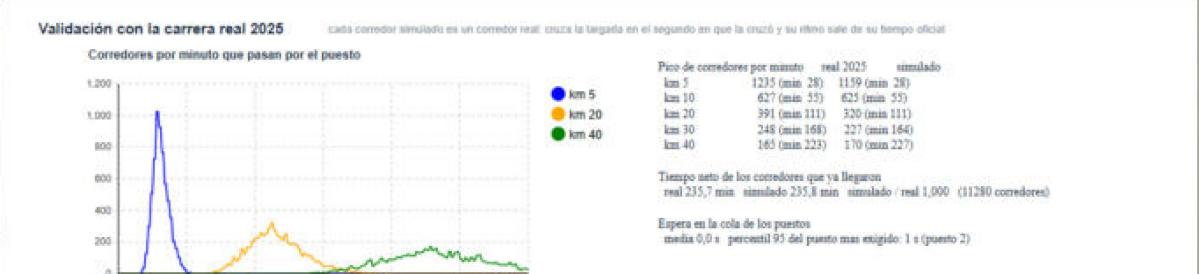
\includegraphics[width=0.95\textwidth]{figuras_tpi/cap_validacion.png}
    \caption{Sección de validación del modelo al final de una corrida del escenario base.}
\end{figure}

\end{document}
